\subsubsection{Logic contracts}
In this section are illustrated the logic contracts of \textit{Soldino}, these contracts implement a substantial part of the business logic, in fact they define inputs validation mechanics, events to be emitted on the blockchain when a state change is made and comunicate with each other.
For the comunication part, since logic contracts are upgradeable, every logic contract has a \texttt{ContractManager} state variable, used to get the latest address of another contract. In this way the coupling between logic contract is minimum and there's no need to maintain correct references in each logic contract.\\
However
\paragraph{UserLogic}\mbox{}\\
\begin{figure}[H]
	\centering
	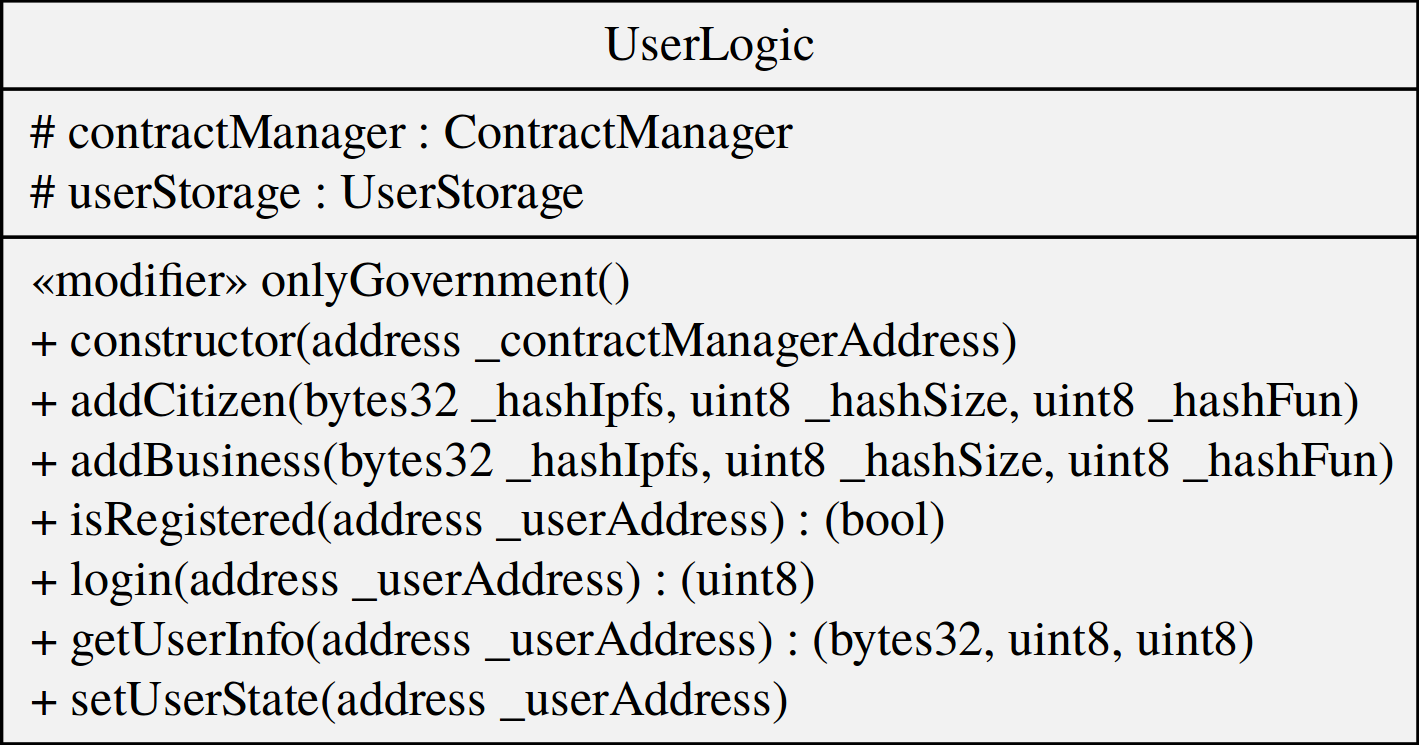
\includegraphics[scale=0.20]{res/images/solidity/userlogic.png}
	\caption{class diagram of the UserLogic contract}
\end{figure}

\paragraph{ProductLogic}\mbox{}\\
\begin{figure}[H]
	\centering
	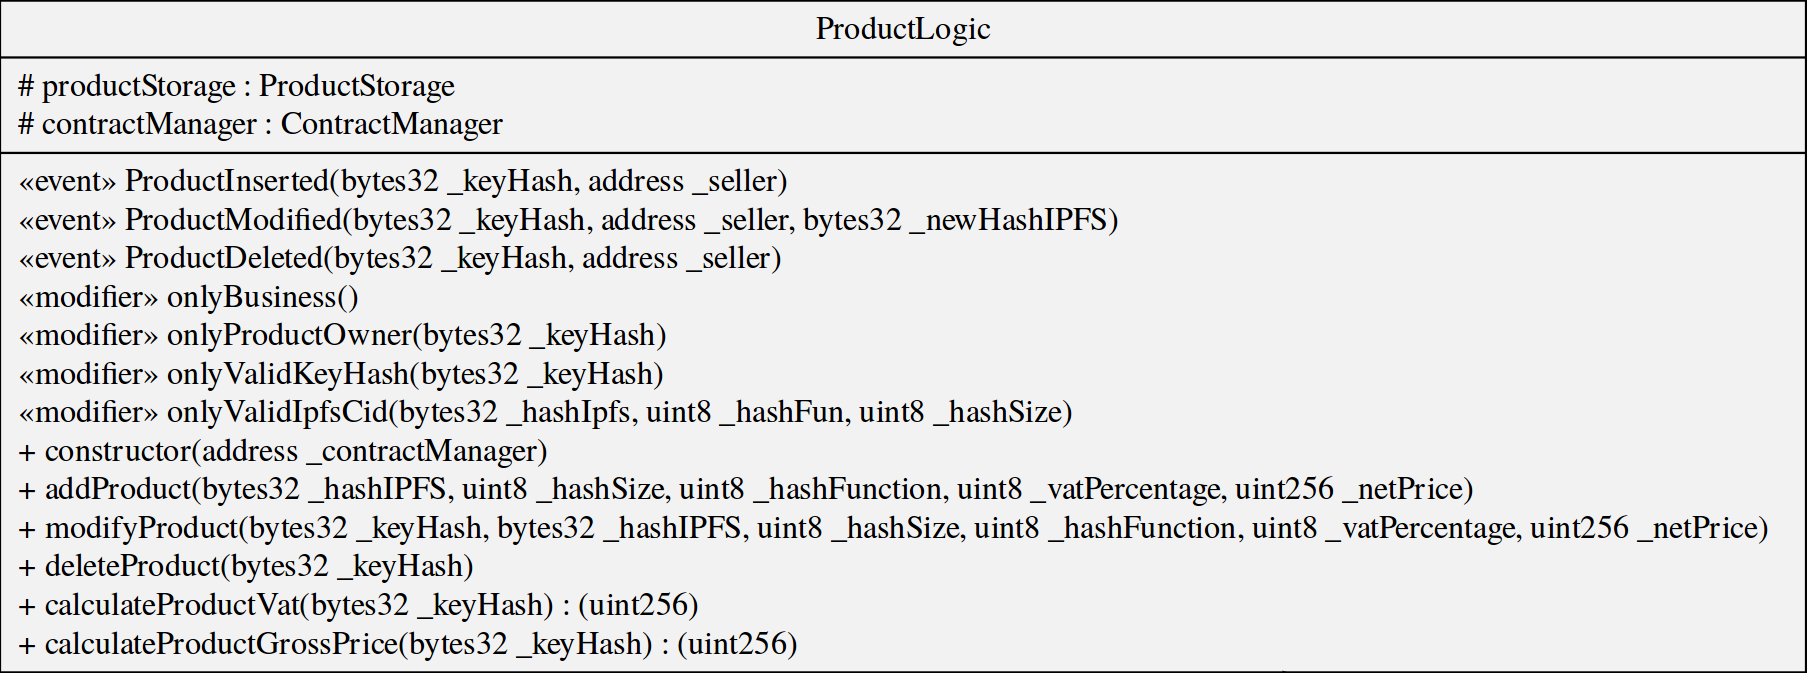
\includegraphics[scale=0.25]{res/images/solidity/productlogic.png}
	\caption{class diagram of the ProductLogic contract}
\end{figure}

\paragraph{VatLogic}\mbox{}\\
\begin{figure}[H]
	\centering
	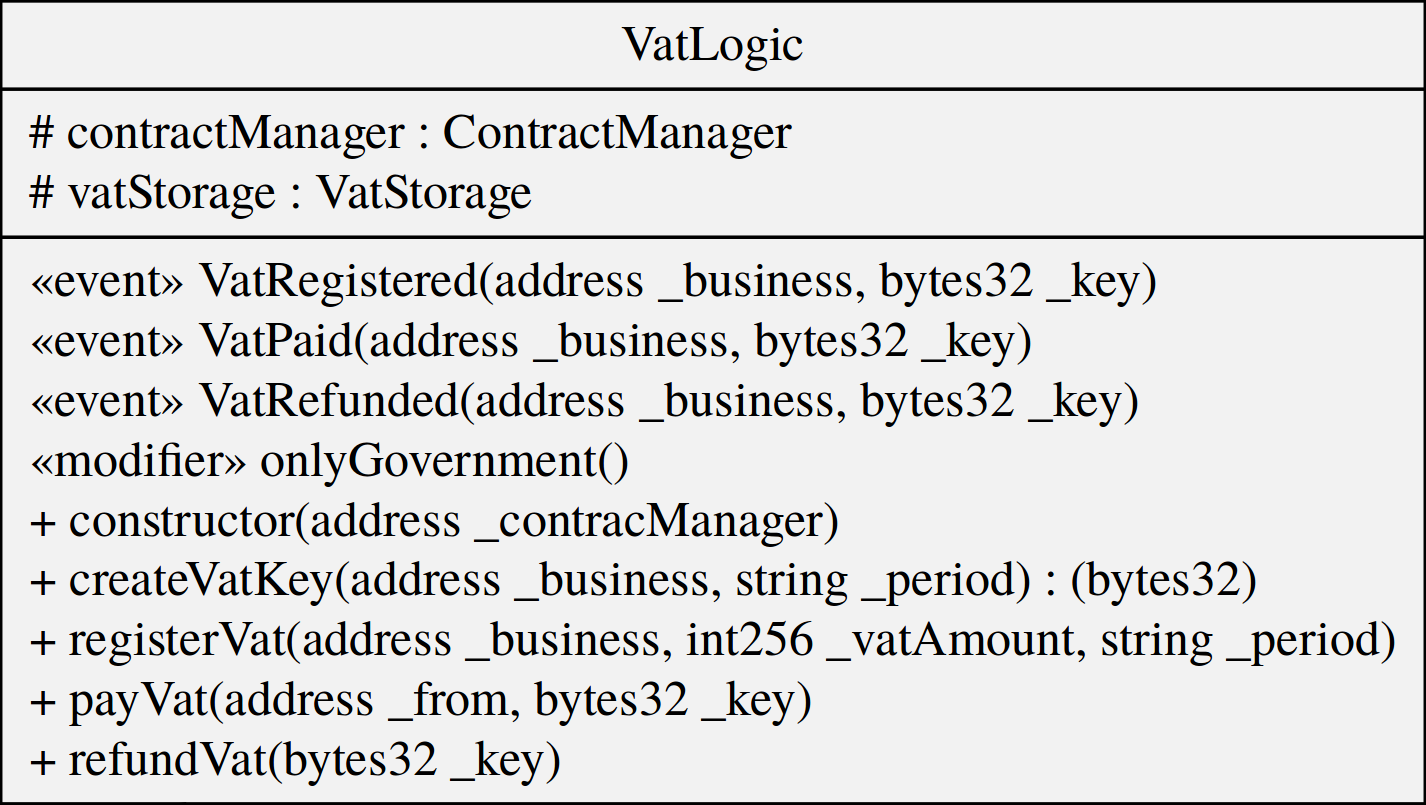
\includegraphics[scale=0.20]{res/images/solidity/vatlogic.png}
	\caption{class diagram of the VatLogic contract}
\end{figure}

\paragraph{OrderLogic}\mbox{}\\
\begin{figure}[H]
	\centering
	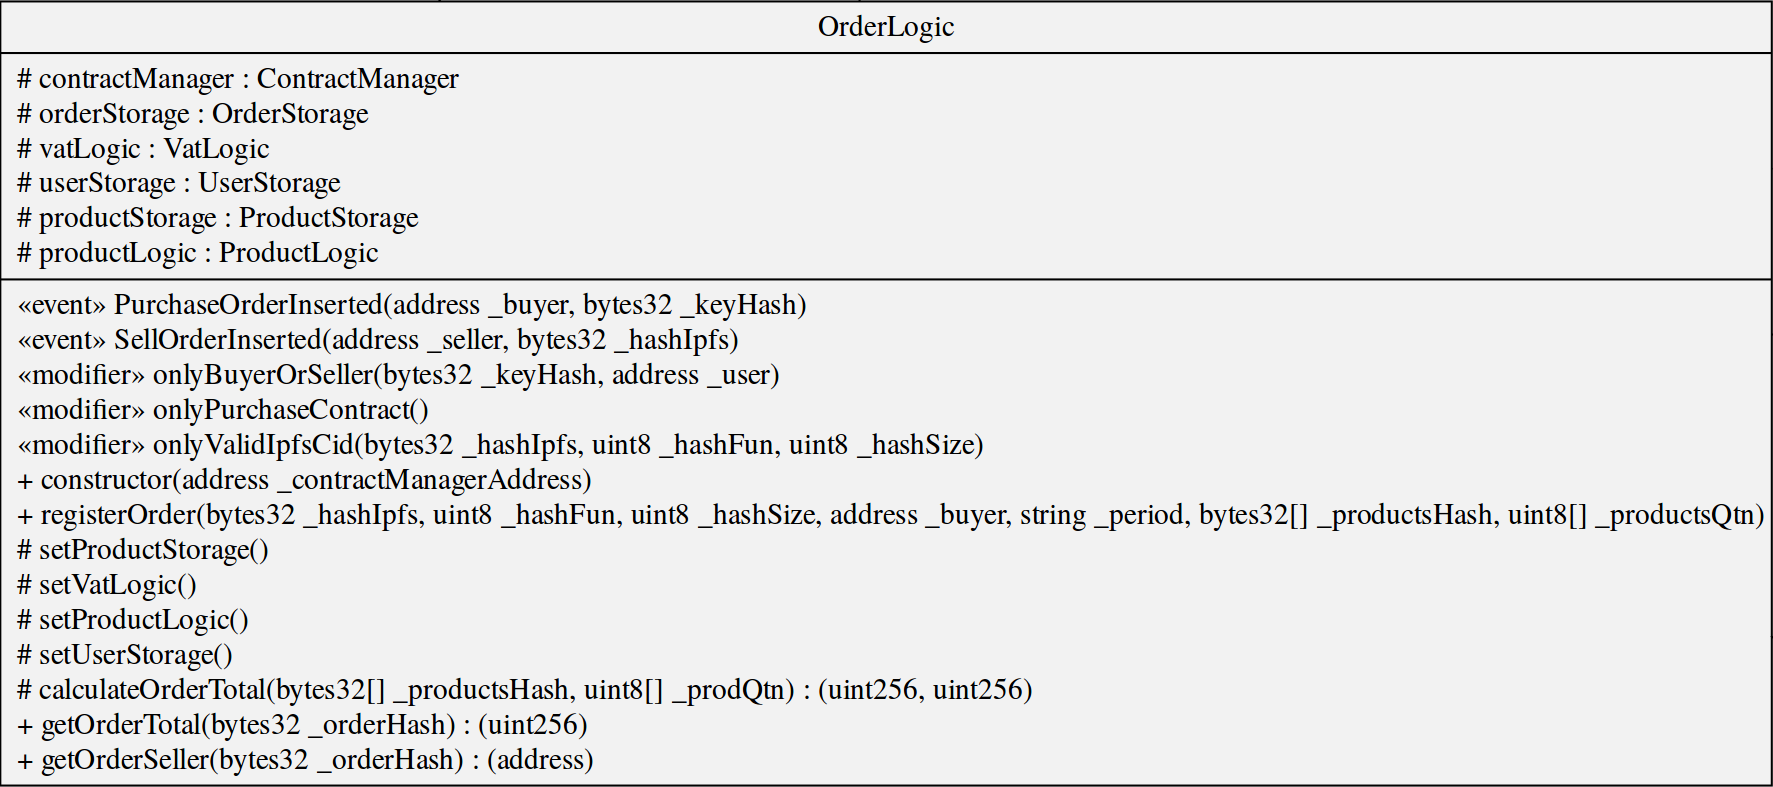
\includegraphics[scale=0.25]{res/images/solidity/orderlogic.png}
	\caption{class diagram of the OrderLogic contract}
\end{figure}